% Strain_OutdoorsResponse2Controls.tex

\resizebox{!}{0.45\textwidth}{
	\begin{tikzpicture}
		\node[anchor=south west,inner sep=0] (image) at (0,0)%
			{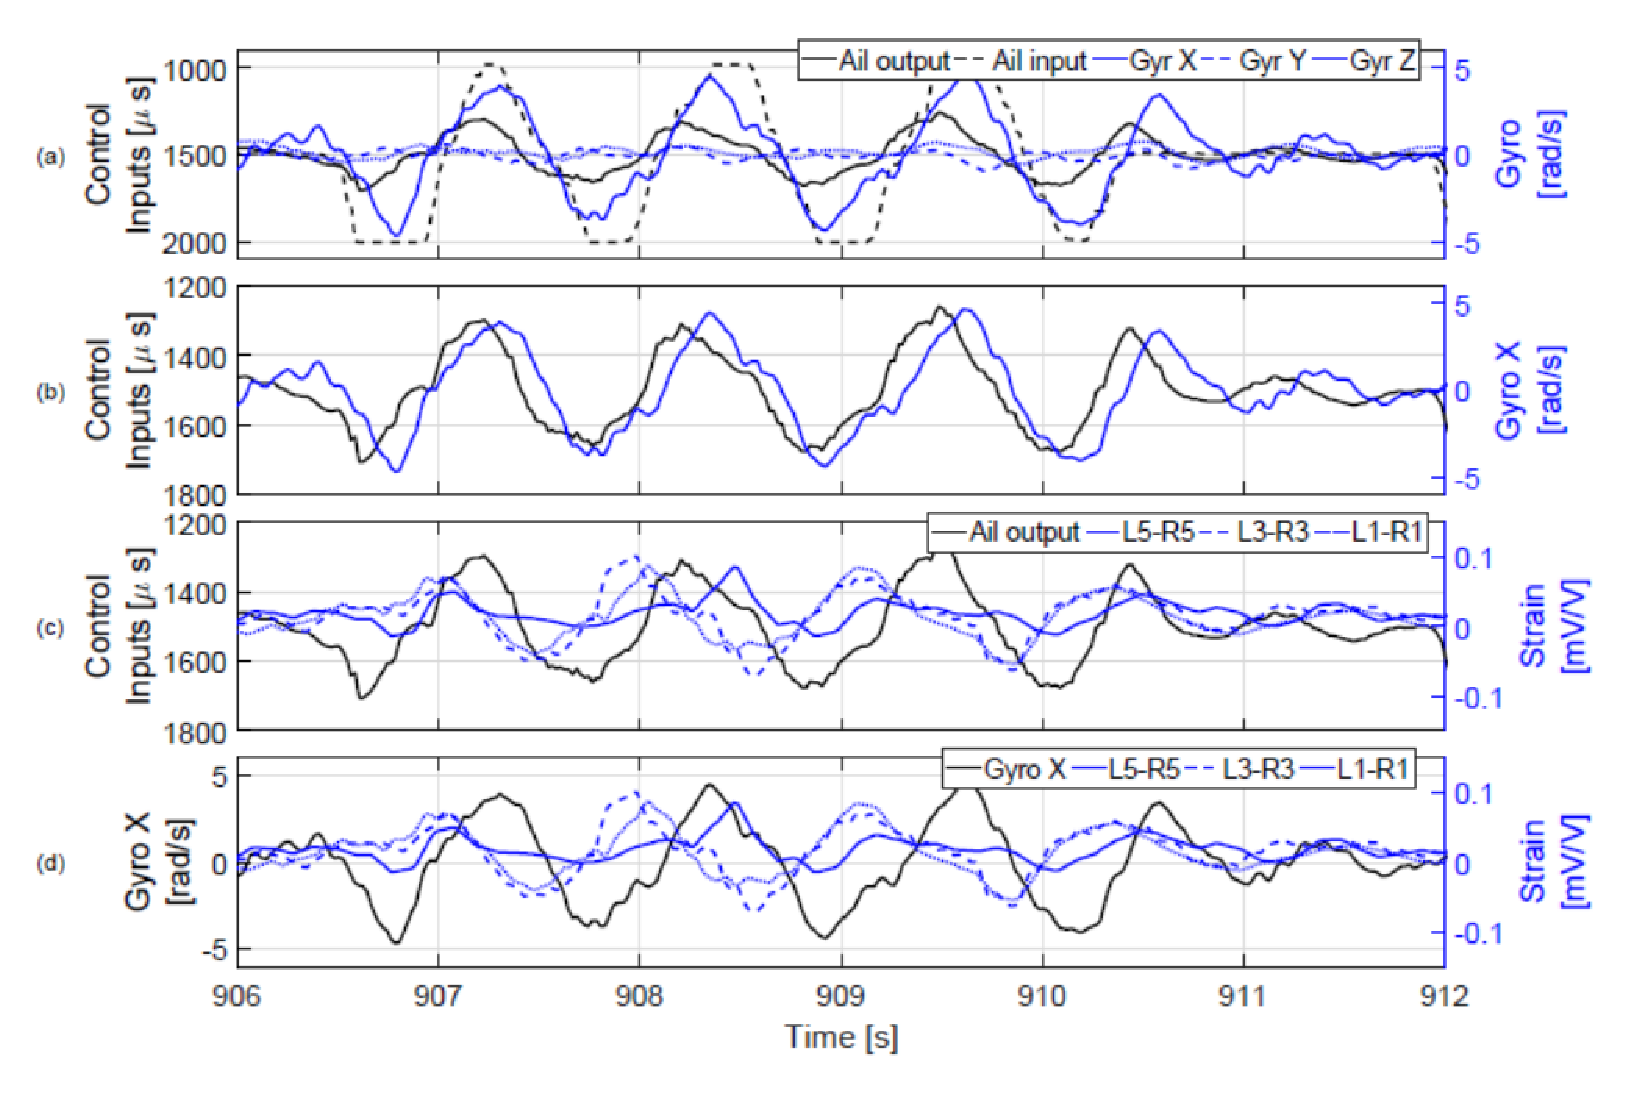
\includegraphics[width=\textwidth]{Strain_OutdoorsResponse2Controls.eps}};
		% Define scope with 'image' dimensions as reference
		\begin{scope}[x={(image.south east)},y={(image.north west)}]
			\draw[help lines,xstep=.05,ystep=.05] (0,0) grid (1,1);
			\foreach \x in {0,1,...,9} { \node [anchor=north] at (\x/10,0) {0.\x}; }
			\foreach \y in {0,1,...,9} { \node [anchor=east] at (0,\y/10) {0.\y}; }
			
		\end{scope}
  \end{tikzpicture}
}